\subsection{Kỹ thuật word2vec}
\textit{word2vec} là một trong những kỹ thuật được sử dụng phổ biến nhất trong lĩnh vực \textit{Xử lý ngôn ngữ tự nhiên}. \textit{word2vec} được tạo ra và công bố vào năm 2013 bởi một nhóm các nhà nghiên cứu dẫn đầu bởi Tomas Mikolov ở Google và đã được đăng ký bảo hộ quyền phát minh sáng chế.

Kỹ thuật \textit{word2vec} đã giải quyết vấn đề tương quan ngữ nghĩa của mô hình Auto-Encoder khi biến đổi các từ trong một \textit{kho ngữ liệu} (corpus) thành các vector bằng cách dựa vào \textit{thông tin ngữ cảnh} (contextual information) của chúng trong \textit{kho ngữ liệu} đó. Bởi vậy, mô hình sẽ học để sinh ra các vector tương tự nhau cho những từ có ngữ cảnh tương tự nhau.

\textit{Thông tin ngữ cảnh} của một \textit{từ mục tiêu} (focus word) là một \textit{cửa sổ} (window) chứa các từ ở bên trái và bên phải của \textit{từ mục tiêu}, được gọi là các \textit{từ ngữ cảnh} (context word). Ta nói \textit{kích thước cửa sổ} (window size) = $k$ khi \textit{cửa sổ} này chứa $k$ từ bên trái và $k$ từ bên phải của \textit{từ mục tiêu}. Ta xét một ví dụ đơn giản sau:

\begin{exmp}
\label{ex:skip-gram-corpus}
\hrulefill\\
Giả sử \textit{kho ngữ liệu} của ta gồm 3 tài liệu D1, D2, D3:

	D1: \textit{Hôm qua tôi đi học.}

    D2: \textit{Hôm nay tôi cũng đi học}

    D3: \textit{Ngày mai tôi không đi học.}

Sau bước tiền xử lý, \textit{kho ngữ liệu} trên sẽ được biến đổi thành tập các từ phân biệt được sắp xếp theo thứ tự bảng chữ cái như sau: \{\textit{cũng, đi, học, hôm\_nay, hôm\_qua, không, ngày\_mai, tôi}\}.

Với \textit{kích thước cửa sổ} = 1, ta có \textit{thông tin ngữ cảnh} của các từ trong tài liệu D1 như sau:

\begin{table}[!h]
\centering
\begin{tabular}{|l|l|}
\hline
\textbf{Từ mục tiêu} & \textbf{Từ ngữ cảnh} \\ \hline
hôm\_qua             & tôi                  \\ \hline
tôi                  & hôm\_qua, đi         \\ \hline
đi                   & tôi, học             \\ \hline
học                  & đi                   \\ \hline
\end{tabular}
\caption{Từ mục tiêu và ngữ cảnh tương ứng của D1 khi kích thước cửa sổ = 1}
\label{tab:window-size-1}
\end{table}

Với \textit{kích thước cửa sổ} = 2, ta có \textit{thông tin ngữ cảnh} của các từ trong tài liệu D1 như sau:

\begin{table}[ht]
\centering
\begin{tabular}{|l|l|}
\hline
\textbf{Từ mục tiêu} & \textbf{Từ ngữ cảnh} \\ \hline
hôm\_qua             & tôi, đi              \\ \hline
tôi                  & hôm\_qua, đi, học    \\ \hline
đi                   & hôm\_qua, tôi, học   \\ \hline
học                  & tôi, đi              \\ \hline
\end{tabular}
\caption{\textit{Từ mục tiêu} và \textit{từ ngữ cảnh} tương ứng của D1 khi \textit{kích thước cửa sổ} = 2}
\label{tab:window-size-2}
\end{table}

\end{exmp}

Tương tự như kỹ thuật \textit{Auto-Encoder}, \textit{word2vec} cũng sử dụng một mạng nơ-ron ba lớp. Điểm khác biệt ở đây là đối với kỹ thuật \textit{Auto-Encoder}, \textit{đầu vào} (input) và \textit{đầu ra} (output) cùng là một \textit{từ mục tiêu}, còn đối với kỹ thuật \textit{word2vec} ta sẽ dùng \textit{từ mục tiêu} và các \textit{từ ngữ cảnh} của nó để làm đầu vào và đầu ra. Tuỳ thuộc vào cách ta sử dụng \textit{từ mục tiêu} để làm đầu vào hay đầu ra, mà có hai mô hình \textit{word2vec} khác nhau là \textit{skip-gram} và \textit{CBOW} (Continuous Bag of Words). Ta sẽ nói rõ chi tiết hai mô hình này ở phần sau.

\subsubsection{Skip-gram}
Ở mô hình \textit{skip-gram}, ta sẽ sử dụng \textit{từ mục tiêu} làm đầu vào và đầu ra mong đợi là \textit{từ ngữ cảnh} để \textit{huấn luyện} (train) mạng nơ-ron. Như vậy mỗi \textit{mẫu} (sample) huấn luyện sẽ là một cặp (\textit{từ mục tiêu}, \textit{từ ngữ cảnh}) và tập dữ liệu huấn luyện của ta sẽ bao gồm tất cả các cặp từ trong \textit{kho ngữ liệu}.

Xét \textit{kho ngữ liệu} bao gồm ba tài liệu D1, D2, D3 như ở ví dụ trước. Để huấn luyện mô hình skip-gram, đầu tiên ta đưa đầu vào là \textit{tôi} và đầu ra mong đợi là \textit{hôm\_nay}. Tiếp tục đưa đầu vào \textit{tôi} và đầu ra mong đợi là từ \textit{đi}.  Tương tự như vậy cho tất cả các cặp từ khác trong \textit{kho ngữ liệu}.

Với \textit{kích thước cửa sổ} = 1, ta có sơ đồ huấn luyện mô hình skip-gram như sau:

\begin{figure}[!h]
	\centering
		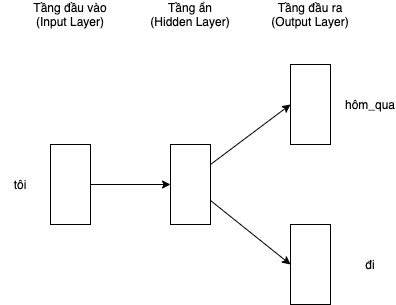
\includegraphics[width=0.5\columnwidth]{books/artificial-neural-network/chapter04/figure/skip-gram-window-size-1.jpg}
        \caption{Sơ đồ huấn luyện mô hình skip-gram khi \textit{kích thước cửa sổ} là 1}
        \label{fig:skip_gram_window_size_1}
\end{figure}

Với \textit{kích thước cửa sổ} = 2, ta có sơ đồ huấn luyện mô hình skip-gram như sau:
\clearpage
\begin{figure}[!h]
	\centering
		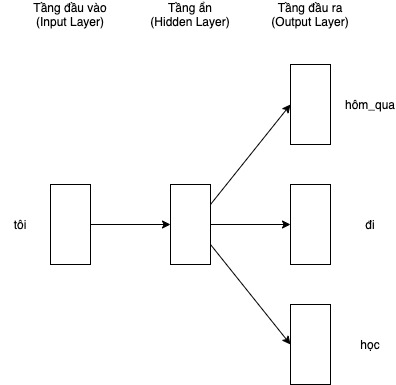
\includegraphics[width=0.5\columnwidth]{books/artificial-neural-network/chapter04/figure/skip-gram-window-size-2.jpg}
        \caption{Sơ đồ huấn luyện mô hình skip-gram khi kích thước cửa sổ là 2}
        \label{fig:skip_gram_window_size_2}
\end{figure}

Để ý khi \textit{kích thước cửa sổ} = 2, do \textit{từ mục tiêu} là \textit{tôi} chỉ có một từ phía bên trái và hai từ phía bên phải, nên ta chỉ có 3 cặp từ. Trong trường hợp \textit{từ mục tiêu} có đầy đủ \textit{từ ngữ cảnh}, ta sẽ 4 cặp từ để huấn luyện (2 \textit{từ ngữ cảnh} bên trái và 2 \textit{từ ngữ cảnh} bên phải), minh hoạ bằng tài liệu D2 như hình ~\ref{fig:skip_gram_window_size_2_full}

\begin{figure}[!h]
	\centering
		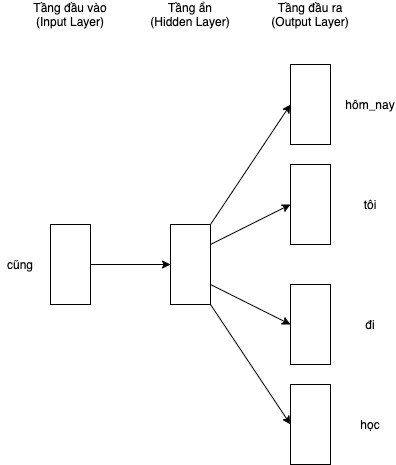
\includegraphics[width=0.5\columnwidth]{books/artificial-neural-network/chapter04/figure/skip-gram-window-size-2-full.jpg}
        \caption{Sơ đồ huấn luyện mô hình skip-gram khi \textit{kích thước cửa sổ} là 2 và sử dụng \textit{từ mục tiêu} trong tài liệu D2}
        \label{fig:skip_gram_window_size_2_full}
\end{figure}

Trong trường hợp tổng quát, khi \textit{kích thước cửa sổ} = $k$, thì với mỗi từ mục tiêu ta có khoảng $2k$ cặp từ để đưa vào huấn luyện mạng nơ-ron skip-gram.

\subsubsection{Xây dựng mô hình mạng nơ-ron skip-gram}
Tương tự như kỹ thuật Auto-Encoder, mô hình skip-gram cũng sử dụng mạng nơ-ron 3 lớp gồm \textit{tầng đầu vào} (input layer), \textit{tầng ẩn} (hidden layer) và \textit{tầng đầu ra} (output layer). Để đơn giản ta xét \textit{kho ngữ liệu} chỉ bao gồm 3 tài liệu D1, D2, D3 như ở ví dụ trên. Khi đó, mạng nơ-ron sẽ có dạng như hình \ref{fig:skip_gram}.

\begin{figure}[!h]
	\centering
		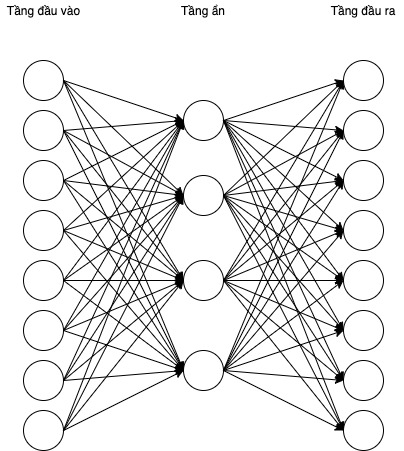
\includegraphics[width=0.5\columnwidth]{books/artificial-neural-network/chapter04/figure/skip-gram-architecture.jpg}
        \caption{Sơ đồ minh hoạ mạng nơ-ron skip-gram}
        \label{fig:skip_gram}
\end{figure}

Ở mô hình này, chúng ta không sử dụng \textit{hàm kích hoạt} (activation function) cho \textit{tầng ẩn} (hidden layer) như các mạng nơ-ron thông thường. \textit{Tầng đầu ra} (output layer) sẽ sử dụng \textit{hàm kích hoạt} là \textit{softmax}. Ta sẽ lần lượt tìm hiểu chi tiết về các tầng này ở phần sau.

\subsubsection{Tầng đầu vào (Input layer)}
Tương tự như kỹ thuật Auto-Encoder, ta cũng biểu diễn một từ thành một vector one-hot để làm đầu vào của mạng nơ-ron. \textit{Kho ngữ liệu} gồm D1, D2, D3 trên có 8 \textit{từ phân biệt} (unique word) nên mỗi từ sẽ được biễn bằng một vector one-hot có 8 chiều, trong đó chỉ có chiều ở vị trí tương ứng với vị trí của từ trong \textit{kho ngữ liệu} bằng 1, còn tất cả các chiều khác đều bằng 0. Vậy \textit{tầng đầu vào} sẽ có 8 nơ-ron tương ứng với vector one-hot 8 chiều đó. Bằng cách biểu diễn như trên, ta được các vector one-hot sau:

\textit{cũng} = $\begin{bmatrix}
        1 & 0 & 0 & 0 & 0 & 0 & 0 & 0
    \end{bmatrix}$

\textit{đi} = $\begin{bmatrix}
        0 & 1 &0 & 0 & 0 & 0 & 0 & 0
    \end{bmatrix}$

\textit{học} = $\begin{bmatrix}
        0 & 0 & 1 & 0 & 0 & 0 & 0 & 0
    \end{bmatrix}$

\textit{hôm\_nay} = $\begin{bmatrix}
        0 & 0 & 0 & 1 & 0 & 0 & 0 & 0
    \end{bmatrix}$

\textit{hôm\_qua} = $\begin{bmatrix}
        0 & 0 & 0 & 0 & 1 & 0 & 0 & 0
    \end{bmatrix}$

\textit{không} = $\begin{bmatrix}
        0 & 0 & 0 & 0 & 0 & 1 & 0 & 0
    \end{bmatrix}$

\textit{ngày\_mai} = $\begin{bmatrix}
        0 & 0 & 0 & 0 & 0 & 0 & 1 & 0
    \end{bmatrix}$

\textit{tôi} = $\begin{bmatrix}
        0 & 0 & 0 & 0 & 0 & 0 & 0 & 1
    \end{bmatrix}$

Tổng quát, số lượng nơ-ron của \textit{tầng đầu vào} sẽ bằng đúng số lượng các từ phân biệt trọng \textit{kho ngữ liệu} và bằng số chiều của vector one-hot biểu diễn cho mỗi từ. Trong thực tế, kích thước của \textit{kho ngữ liệu} có thể lên đến hàng triệu từ.

\subsubsection{Tầng ẩn (Hidden layer)}
Giả sử mạng nơ-ron cần học 4 \textit{đặc trưng} (feature) của các từ, \textit{tầng ẩn} sẽ bao gồm 4 nơ-ron. Với tầng đầu vào của mô hình là vector one-hot 8 chiều, vậy \textit{ma trận trọng số} (weight matrix) cần phải học của \textit{tầng ẩn} sẽ là $8\times 4$. Chú ý con số 4 đặc trưng của từ là một \textit{siêu tham số} (hyper parameter), ta có thể điều chỉnh giá trị này để đạt được kết quả phù hợp tuỳ theo từng bài toán khác nhau.\\

\begin{table}[!h]
\centering
\begin{tabular}{|l|l|l|l|}
\hline
0.3  & 0.5  & 0.2 & 0.01 \\ \hline
1.2  & 2.4  & 1.5  & 0.2  \\ \hline
2.5  & 1.1  & 0.3  & 0.55 \\ \hline
1    & 0.15 & 0.6  & 2.1  \\ \hline
1.3  & 1.7  & 2.1  & 0.24 \\ \hline
2.2  & 1.8  & 0.6  & 0.3  \\ \hline
1.4  & 0.12 & 0.04 & 2.4  \\ \hline
1.12 & 0.8  & 0.5  & 1.25 \\ \hline
\end{tabular}
\caption{Minh hoạ \textit{ma trận trọng số} của tầng ẩn sau khi huấn luyện xong}
\label{tab:hidden-layer-weight-matrix}
\end{table}

Tổng quát, số lượng nơ-ron của \textit{tầng ẩn} bằng với số lượng đặc trưng mà ta muốn học ở mỗi từ trong \textit{kho ngữ liệu} và cũng là số chiều của vector đầu ra của \textit{tầng ẩn}. Như vậy, nếu muốn mô hình skip-gram biểu diễn các từ thành vector bao nhiêu chiều thì ta sử dụng bấy nhiêu nơ-ron ở \textit{tầng ẩn}. Trong thực tế, số lượng nơ-ron của \textit{tầng ẩn} thường vào khoảng vài trăm. Sau khi huấn luận xong, ta sẽ giữ lại \textit{ma trận trọng số} để dùng cho mục đích biến đổi từ thành vector. Giả sử \textit{kho ngữ liệu} có $V$ từ phân biệt và ta muốn biến đổi từ thành vector có $N$ chiều thì \textit{ma trận trọng số} của mạng nơ-ron skip-gram sẽ có kích thước là $V\times N$. Khi đó mỗi từ (được biểu diễn bằng vector one-hot $1\times V$) sẽ được biến đổi thành một vector $1\times N$, vector này sẽ là một hàng trong \textit{ma trận trọng số}.

\subsubsection{Tầng đầu ra (Output layer)}
Tiếp tục xét \textit{kho ngữ liệu} D1, D2, D3 ở trên, \textit{tầng đầu ra} của mô hình skip-gram sẽ có số lượng nơ-ron đúng bằng số lượng nơ-ron của \textit{tầng đầu vào}, tức là 8 nơ-ron. \textit{Tầng đầu ra} cũng có một \textit{ma trận trọng số} để học có kích thước $4\times 8$, để biến đổi vector $1\times 4$ của \textit{tầng ẩn} thành vector $1\times 8$ đầu ra. Sau khi huấn luyện mạng nơ-ron xong, toàn bộ \textit{tầng đầu ra} và \textit{ma trận trọng số} này sẽ bị loại bỏ.

\begin{table}[!h]
\centering
\begin{tabular}{|l|l|l|l|l|l|l|l|}
\hline
0.3 & 0.5  & 0..2 & 0.01 & 0.23 & 1    & 1.24 & 0.17 \\ \hline
1.2 & 2.4  & 1.5  & 0.2  & 2.5  & 1.17 & 0.05 & 0.26 \\ \hline
2.5 & 1.1  & 0.3  & 0.55 & 1.3  & 0.35 & 1.34 & 1.36 \\ \hline
1   & 0.15 & 0.6  & 2.1  & 2.8  & 0.68 & 0.87 & 2.1  \\ \hline
\end{tabular}
\caption{Minh hoạ \textit{ma trận trọng số} của tầng đầu ra sau khi huấn luyện xong}
\end{table}

\subsubsection{Kết quả}
Giả sử sau khi huấn luyện xong ta được \textit{ma trận trọng số} của \textit{tầng ẩn} như ở bảng \ref{tab:hidden-layer-weight-matrix}. Dùng mạng nơ-ron skip-gram này để biến đổi thì mỗi từ thành một vector như sau:

\textit{cũng} = $\begin{bmatrix}
        0.3 & 0.5 & 0.2 & 0.01
    \end{bmatrix}$

\textit{đi} = $\begin{bmatrix}
        1.2 & 2.4 & 1.5 & 0.2
    \end{bmatrix}$

\textit{học} = $\begin{bmatrix}
        2.5 & 1.1 & 0.3 & 0.55
    \end{bmatrix}$

\textit{hôm\_nay} = $\begin{bmatrix}
        1 & 0.15 & 0.6 & 2.1
    \end{bmatrix}$

\textit{hôm\_qua} = $\begin{bmatrix}
        1.3 & 1.7 & 2.1 & 0.24
    \end{bmatrix}$

\textit{không} = $\begin{bmatrix}
        2.2 & 1.8 & 0.6 & 0.3
    \end{bmatrix}$

\textit{ngày\_mai} = $\begin{bmatrix}
        1.4 & 0.12 & 0.04 & 2.4
    \end{bmatrix}$

\textit{tôi} = $\begin{bmatrix}
        1.12 & 0.8 & 0.5 & 1.12
    \end{bmatrix}$

Để ý thấy rằng những từ có ngữ cảnh tương tự nhau thì sẽ cho ra các vector tương tự nhau.

\subsubsection{Tổng kết mô hình skip-gram}
Mô hình skip-gram sử dụng mạng nơ-ron 3 lớp tương tự như kỹ thuật Auto-Encoder nhưng thay vì sử dụng \textit{từ mục tiêu} cho cả đầu vào và đầu ra thì sử dụng các \textit{từ ngữ cảnh} làm đầu ra để huấn luyện. Vì vậy, ngoài việc thu giảm số chiều của vector biểu diễn từ, thì mô hình skip-gram đã giải quyết nhược điểm của mô hình Auto-Encoder, tức là đã giữ lại được ngữ nghĩa của các từ trong \textit{kho ngữ liệu}. Các từ có ngữ cảnh tương tự nhau sẽ được biến đổi thành thành các vector tương tự nhau.

\subsubsection{CBOW (Continuous Bag of Words)}
CBOW có input là từ mục tiêu (focus word), output là các từ trong ngữ cảnh  (context). Ý tưởng chính của mô hình CBOW là dự đoán từ mục tiêu dựa vào các từ ngữ cảnh xung quanh nó trong một phạm vi nhất định. Cho từ mục tiêu $w_{t}$ tại vị trí $t$ trong câu văn bản, khi đó đầu vào là các từ ngữ cảnh $(w_{t-m}, ..., w_{t-1}, w_{t+1}, ..., w_{t+m})$ xung quanh từ $w_{t}$ trong phạm vi $m$.
\clearpage
\begin{figure}[ht]
	\centering
		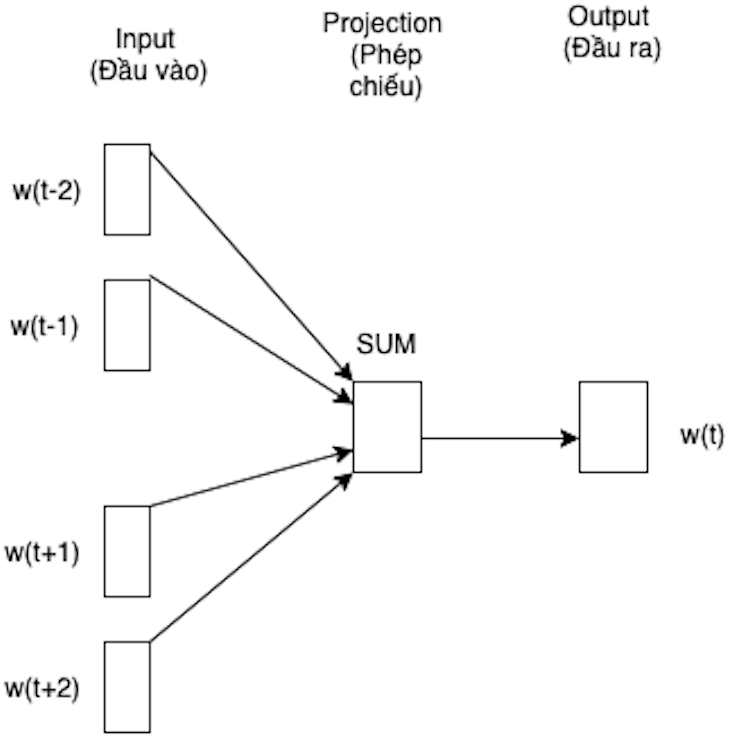
\includegraphics[width=0.5\columnwidth]{books/artificial-neural-network/chapter04/figure/cbow_1.png}
        \caption{Sơ đồ minh hoạ CBOW }
        \label{fig:cbow1}
\end{figure}

Ví dụ: \textbf{"Hôm nay tôi cũng đi học"}
\begin{figure}[!htb]
	\centering
		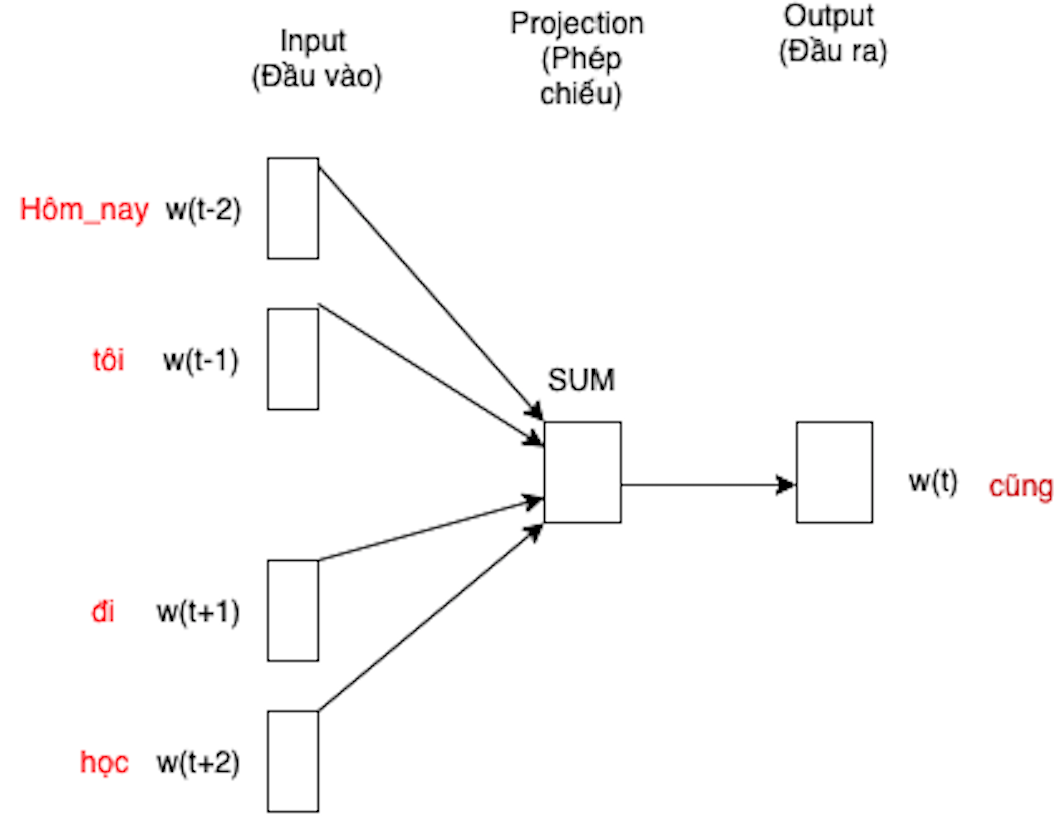
\includegraphics[width=0.5\columnwidth]{books/artificial-neural-network/chapter04/figure/cbow_3.png}
        \caption{Sơ đồ minh hoạ CBOW với ví dụ trên}
        \label{fig:cbow2}
\end{figure}

Mô hình CBOW tổng quát được minh hoạ trong Hình \ref{fig:cbow3} với kích thước đầu vào gồm \textbf{C} từ ngữ cảnh, \textbf{V} là kích thước của tập từ vựng và hyperparameter \textbf{N} là kích thước của tầng hidden (hidden layer). Các unit thuộc layer kế cận được kết nối theo kiểu fully connected.
\clearpage
\begin{figure}[!h]
    \centering
    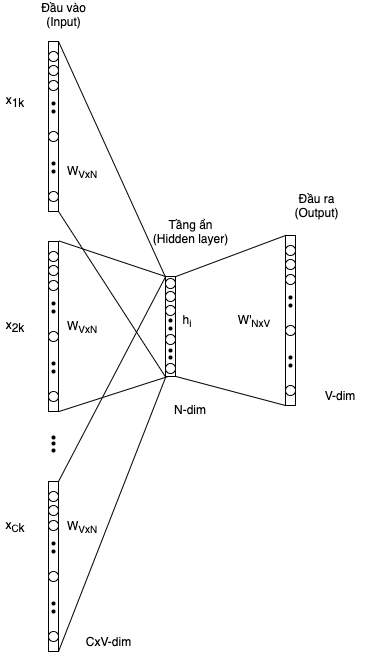
\includegraphics[width=0.5\columnwidth]{books/artificial-neural-network/chapter04/figure/cbow_4.png}
    \caption{Mô hình CBOW dạng tổng quát}
    \label{fig:cbow3}
\end{figure}

Mỗi từ đầu vào ở vị trí thứ $k$ trong từ vựng được biểu diễn bằng một vector one-hot dưới dạng:
\begin{center}
    $x^{k}$ =
    $\begin{bmatrix}
        x_{1}\\
        x_{2} \\
        \vdots \\
        x_{k} \\
        \vdots \\
        x_{V} \\
    \end{bmatrix}$
\end{center}

Với mỗi vector $x^{k}$ chỉ có một phần tử $x_{k}$ có giá trị 1, các phần tử còn lại có giá trị 0.

Ma trận trọng số giữa tầng input (input layer) và tầng hidden $W$ kích thước $V\times N$ được biểu diễn như sau:
\begin{center}
    $W_{V\times N}$ =
    $\begin{bmatrix}
        w_{11} & w_{12} & \dots & w_{1N}\\
        w_{21} & w_{22} & \dots & w_{2N} \\
        \vdots & \vdots & \ddots & \vdots \\
        w_{V1} & w_{V2} & \dots & w_{VN}
    \end{bmatrix}$
\end{center}

Mỗi hàng của ma trận \textbf{W}  là một biểu diễn vector có số chiều là \textbf{N} tương ứng với một từ \textbf{w} trong tập từ vựng.

Với mỗi vector $x^{k}$, ta có:
\begin{center}
    \begin{equation}
        \begin{split}
            W^T x^{k} & =
            \begin{bmatrix}
            w_{11} & w_{12} & \dots & w_{1V}\\
            w_{21} & w_{22} & \dots & w_{2V} \\
            \vdots & \vdots & \ddots & \vdots \\
            w_{N1} & w_{N2} & \dots & w_{NV}
        \end{bmatrix}
        \begin{bmatrix}
            x_{1}\\
            x_{2} \\
            \vdots \\
            x_{k} \\
            \vdots \\
            x_{V} \\
        \end{bmatrix} \\
         & =
        \begin{bmatrix}
            w_{k1}x_{k}\\
            w_{k2}x_{k} \\
            \vdots \\
            w_{kN}x_{k} \\
        \end{bmatrix} \\
         & =
        \begin{bmatrix}
            w_{k1}\\
            w_{k2} \\
            \vdots \\
            w_{kN} \\
        \end{bmatrix} \\
         & = v^T_{k}
        \end{split}
    \end{equation}
\end{center}

Ma trận $h$ có kích thước $N\times 1$ được biểu diễn như sau:

\begin{center}
    \begin{equation}
    \begin{split}
        h & = \frac{1}{C} \times W^T \left( x^{(1)} + x^{(2)} + \dots + x^{(C)} \right) \\
        & = \frac{1}{C} \times \left( v^T_{1} + v^T_{2} + \dots + v^T_{C} \right) \\
        & = \frac{1}{C} \times \left( v_{1} + v_{2} + \dots + v_{C} \right)^T
    \end{split}
    \end{equation}
\end{center}

Từ tầng hidden đến tầng output (output layer) là các trọng số được biểu diễn bằng một ma trận $W'$ với kích thước $N\times V$ có dạng như sau:
\begin{center}
    $W'_{N\times V}$ =
    $\begin{bmatrix}
        w'_{11} & w'_{12} & \dots & w'_{1V}\\
        w'_{21} & w'_{22} & \dots & w'_{2V} \\
        \vdots & \vdots & \ddots & \vdots \\
        w'_{N1} & w'_{N2} & \dots & w'_{NV}
    \end{bmatrix}$
\end{center}

Kết quả của tầng hidden sẽ được map với đầu ra chính là trọng số của từng từ có trong V, trọng số càng cao có nghĩa là xác suất từ đó là từ tiếp theo (positive prediction) càng cao. Do trọng số ở tầng output có biên độ không cố định nên thường thì người ta dùng softmax ở đoạn này nhằm  đổi trọng số của output layer thành xác suất (probability).

Chúng ta sẽ tính điểm số cho mỗi từ thứ $j$ trong V theo công thức:
\begin{center}
    $p_{j} = v'^T_{wj}h$
\end{center}

Trong đó $v'_{wj}$ là vector cột thứ $j$ của ma trận $W'$. Hàm $softmax$ để chuẩn hoá phân phối hậu nghiệm của mỗi tập từ vựng như sau:
\begin{center}
    \begin{equation}
        p\left( w_{O} | w_{I,1},w_{I,2}, ..., w_{I,C} \right) = y_{j} = \frac{exp(u_{j})}{\sum_{j'}^{V}exp(u_{j'})}
    \end{equation}
\end{center}

Trong đó $y_{j}$ chính là output của unit thứ $j$ trong tầng output, $w_{O}$ là từ mục tiêu, $w_{I,1} , ..., w_{I, C}$ là các từ ngữ cảnh. Mục tiêu của quá trình huấn luyện là điều chỉnh các trọng số để cực đại hoá hàm phân phối bên trên đối với từ $w_{O}$ và các từ ngữ cảnh $w_{I, 1}, ..., w_{I, C}$ cho trước.
\begin{center}
    $max\left( p\left( w_{O} | w_{I,1},w_{I,2}, ..., w_{I,C} \right) \right) = max\left( log\left( p\left( w_{O} | w_{I,1},w_{I,2}, ..., w_{I,C} \right) \right) \right)$ \\ = $min\left( -log\left( p\left( w_{O} | w_{I,1},w_{I,2}, ..., w_{I,C} \right) \right) \right) = min(E) $
\end{center}

Với $E$ là hàm lỗi cần được cực tiểu hoá, có công thức như sau:
\begin{center}
    \begin{equation}
    \begin{split}
        E & = -log\left( p\left( w_{O} | w_{I,1},w_{I,2}, ..., w_{I,C} \right) \right) \\
        & = -u_{j^*} + log\left( \sum_{j'=1}^{V}exp\left( u_{j'} \right) \right) \\
        & = -v'^T_{wO} h + log\left( \sum_{j'=1}^{V}exp\left( v'^T_{wO} h \right) \right)
    \end{split}
    \end{equation}
\end{center}

Trong đó $j^*$ là vị trí của từ mục tiêu ở tầng output. Phương trình cập nhật trọng số từ tầng hidden đến tầng output như sau:
\begin{center}
    \begin{equation}
        v_{wj'}^{new} = v_{wj'}^{old} - \eta \times \frac{\partial E}{\partial u_{j}} \times h \quad \textrm{với} \; j = 1, 2, ..., V
    \end{equation}
\end{center}

Phương trình cập nhật trọng số từ tầng input đến tầng hidden như sau:
\begin{center}
    \begin{equation}
        v_{w_{c}}^{new} = v_{w_{c}}^{old} - \frac{1}{C} \times \eta \times \left( \frac{\partial E}{\partial h_{i}} \right)^T \quad \textrm{với} \; c = 1, 2, ..., C
    \end{equation}
\end{center}

Trong đó $v_{w_{c}}$ là input vector tương ứng từ thứ c trong C từ ngữ cảnh (context) đầu vào và $\eta$ là learning rate. Sau khi quá trình huấn luyện hoàn tất, chúng ta sẽ thu được 2 ma trận trọng số là $W$ và $W'$.

Với $W'$ có kích thước $N \times V$, ta có:
\begin{center}
    $W'^T_{N\times V}\times h = z$ \\
    $y = softmax(z)$
\end{center}

Nhắc lại, mô hình CBOW cần phải được huấn luyện để điều chỉnh 2 ma trận trọng số $W$ (từ tầng input đến tầng hidden) và $W'$ (từ tầng hidden đến tầng output) sao cho vector $y$ có giá trị xác suất lớn nhất tại vị trí của từ mục tiêu.

Chúng ta sẽ lấy ví dụ để hiểu hơn về cách thức hoạt động của CBOW, cũng với câu \textbf{"Hôm qua tôi đi học"}

Với window size = 1, ta sẽ chọn từ mục tiêu (tầng output) là "đi", và 2 từ ngữ cảnh (tầng input) là "tôi" và "học".

Cho vector one-hot của từ "tôi" và "học" như sau:
\begin{center}
    $x^{toi} =
    \begin{bmatrix}
        0\\
        \textbf{1} \\
        0 \\
        0 \\
        \vdots \\
        0 \\
    \end{bmatrix}$ \\
    \vspace{5mm} %5mm vertical space
    $x^{hoc} =
    \begin{bmatrix}
        0\\
        0\\
        0\\
        \textbf{1} \\
        \vdots \\
        0 \\
    \end{bmatrix}$
\end{center}

Cho ma trận trọng số \textbf{W} có kích thước $V\times N$ sau khi được huấn luyện như sau:
\begin{center}
    $W^T_{V\times N}$ =
    $\begin{bmatrix}
        0.1 & 2.4 & 1.6 & 1.8 & 0.5 & 0.9 & \dots & 3.2 \\
        0.5 & 2.6 & 1.4 & 2.9 & 1.5 & 2.6 & \dots & 6.1 \\
        \vdots & \vdots & \vdots & \vdots & \vdots & \vdots & \ddots & \vdots \\
        0.6 & 1.8 & 2.7 & 1.9 & 2.4 & 3.0 & \dots & 1.2
    \end{bmatrix}$
\end{center}

Ta có:
\begin{center}
    \begin{equation}
    \begin{split}
        v^T_{toi} & = W^T\times x^{toi} \\
        & =
        \begin{bmatrix}
            0.1 & \textbf{2.4} & 1.6 & 1.8 & 0.5 & 0.9 & \dots & 3.2 \\
            0.5 & \textbf{2.6} & 1.4 & 2.9 & 1.5 & 2.6 & \dots & 6.1 \\
            \vdots & \vdots & \vdots & \vdots & \vdots & \vdots & \ddots & \vdots \\
            0.6 & \textbf{1.8} & 2.7 & 1.9 & 2.4 & 3.0 & \dots & 1.2
        \end{bmatrix} \times
        \begin{bmatrix}
            0\\
            \textbf{1} \\
            0 \\
            0 \\
            \vdots \\
            0 \\
        \end{bmatrix} \\
        & =
        \begin{bmatrix}
            \textbf{2.4} \\
            \textbf{2.6} \\
            \vdots \\
            \textbf{1.8} \\
        \end{bmatrix}
    \end{split}
    \end{equation}
\end{center}
\vspace{5mm} %5mm vertical space
\begin{center}
    \begin{equation}
        \begin{split}
            v^T_{hoc} & = W^T\times x^{hoc} \\
            & =
            \begin{bmatrix}
                0.1 & 2.4 & 1.6 & \textbf{1.8} & 0.5 & 0.9 & \dots & 3.2 \\
                0.5 & 2.6 & 1.4 & \textbf{2.9} & 1.5 & 2.6 & \dots & 6.1 \\
                \vdots & \vdots & \vdots & \vdots & \vdots & \vdots & \ddots & \vdots \\
                0.6 & 1.8 & 2.7 & \textbf{1.9} & 2.4 & 3.0 & \dots & 1.2
            \end{bmatrix} \times
            \begin{bmatrix}
                0\\
                \textbf{1} \\
                0 \\
                0 \\
                \vdots \\
                0 \\
            \end{bmatrix} \\
            & =
            \begin{bmatrix}
                \textbf{1.8} \\
                \textbf{2.9} \\
                \vdots \\
                \textbf{1.9} \\
            \end{bmatrix}
        \end{split}
    \end{equation}
\end{center}

Ta tính được $h$ như sau:
\begin{center}
    $h = \left( \frac{v^T_{toi} + v^T_{hoc}}{2} \right)$
\end{center}

Sau khi có được $h$, ta cũng sẽ dùng công thức tính $z$ và $y$ để tìm ra từ mục tiêu gần nhất với các từ input.

Giả sử ta có vector mục tiêu của từ "đi" ở tầng output có kích thước $V\times 1$ như sau:
\begin{center}
    $y =
    \begin{bmatrix}
        0 \\
        0 \\
        0 \\
        0 \\
        0 \\
        \textbf{1} \\
        \vdots \\
        0 \\
    \end{bmatrix}
    $
\end{center}

Quá trình huấn luyện sẽ cho ra vector mục tiêu dưới dạng xác suất của từ "đi" như ví dụ dưới:
\begin{center}
    $y_{training} =
    \begin{bmatrix}
        0.01 \\
        0.02 \\
        0.05 \\
        0.02 \\
        0.03 \\
        \textbf{0.7} \\
        \vdots \\
        0.00 \\
    \end{bmatrix}
    $
\end{center}

\textbf{Chú ý: } khi hiện thực, các vector input trong context sẽ được cộng dồn lại thành một vector có 2N số 1 (với N là số từ đứng trước/đứng sau focus word), để cho ma trận encoder cuối cùng vẫn là một ma trận $N\times V$ như mô hình AE gốc.\\

\textbf{Ưu điểm của CBOW:}
\begin{itemize}
  \item Có bản chất là xác suất cho nên việc hiện thực được cho là vượt trội hơn so với phương pháp khác (nói chung).
  \item Sử dụng ít bộ nhớ.
\end{itemize}

\textbf{Nhược điểm của CBOW:}
\begin{itemize}
  \item CBOW lấy trung bình của ngữ cảnh (context) của 1 từ (ở công thức tính hàm $h$). Ví dụ: Từ "Apple" vừa có thể có nghĩa là "trái cây" lại vừa là "tên của một công ty". CBOW lấy trung bình của 2 contexts và đặt ở giữa.
\end{itemize}

\subsubsection{Bài tập vận dụng word2vec}
\begin{exer}
Sử dụng \textit{kho ngữ liệu} D1, D2, D3 ở ví dụ \ref{ex:skip-gram-corpus}, hãy cho biết \textit{từ mục tiêu} và \textit{từ ngữ cảnh} của các từ trong tài liệu D3 cho hai trường hợp \textit{kích thước cửa sổ} bằng 1 và 2. Chú ý vẽ bảng gồm hai cột \textit{từ mục tiêu} và \textit{từ ngữ cảnh} tương tự như trong ví dụ.
\end{exer}

\begin{exer}
Sử dụng \textit{kho ngữ liệu} D1, D2, D3 ở ví dụ \ref{ex:skip-gram-corpus}, xét \textit{từ mục tiêu} là \textit{tôi} trong tài liệu D3 với \textit{kích thước cửa sổ} = 1. Hãy cho biết khi từ \textit{tôi} được đưa vào huấn luyện thì kiến trúc mạng nơ-ron skip-gram sẽ như thế nào? Giả sử vector sau khi biến đổi có số chiều như trong ví dụ. Chú ý nêu chi tiết số lượng nơ-ron ở mỗi tầng, vẽ mô hình mà nói rõ đầu vào và đầu ra cho mỗi cặp từ.
\end{exer}

\begin{exer}
Sử dụng \textit{kho ngữ liệu} D1, D2, D3 ở ví dụ \ref{ex:skip-gram-corpus}, xét \textit{từ mục tiêu} là \textit{đi}, \textit{hai từ ngữ cảnh} là \textit{tôi} và \textit{học} trong tài liệu D1 với \textit{kích thước cửa sổ} là 1. Hãy cho biết sơ đồ mô hình \textit{CBOW} sẽ như thế nào? Giả sử vector sau khi biến đổi có số chiều như trong ví dụ.
\end{exer}